%%%%%%%%%%%%%%%%%%%%%%%%%%%%%%%%%%%%%%%%%%%%%%%%%%%%%%%%%%%%%%%%%%%%%%
% How to use writeLaTeX: 
%
% You edit the source code here on the left, and the preview on the
% right shows you the result within a few seconds.
%
% Bookmark this page and share the URL with your co-authors. They can
% edit at the same time!
%
% You can upload figures, bibliographies, custom classes and
% styles using the files menu.
%
%%%%%%%%%%%%%%%%%%%%%%%%%%%%%%%%%%%%%%%%%%%%%%%%%%%%%%%%%%%%%%%%%%%%%%

\documentclass[12pt]{article}

\usepackage{sbc-template}

\usepackage{graphicx,url}

\usepackage[brazil]{babel}   
% \usepackage[utf8]{inputenc}  

     
\sloppy

\title{Identificação de sentenças em LLCs}

\author{Henrique Castro e Silva\inst{1}, Leonardo Caetano Gomide\inst{1}}


\address{Departamento de Ciência da Computação - PUC Minas
  \email{leocgomide@gmail.com, henrique.castros@outlook.com}
}

\begin{document} 

\maketitle


\section{Introdução}


No vasto domínio da teoria da computação, as Gramáticas Livres de Contexto (GLCs) emergem como uma ferramenta fundamental para descrever a estrutura sintática de linguagens, abrindo caminho para uma compreensão mais profunda das complexidades inerentes à manipulação de linguagens formais. Enquanto as GLCs desempenham um papel central na modelagem de gramáticas de linguagens de programação, compiladores e processadores de linguagem natural, a exploração das derivações dentro desse contexto torna-se uma área de estudo igualmente crucial.

\section{Algoritmo} \label{sec:firstpage}

O algoritmo CYK (Cocke–Younger–Kasami) nomeado em homenagem a seus 3 inventores independentes na década de 60 é um algoritmo que consegue descobrir se uma sentença \textit{w} é derivada por uma GLC \textit{G}. Ele utiliza da técnica de computação dinâmica para armazenar derivações parciais da sentença até que se obtenha todos os símbolos que podem derivar a sentença inteira, e se o símbolo inicial \textit{s} estiver nesse conjunto, a sentença é derivável pela gramática. O algoritmo tem uma complexidade de $\mathbf{O(n^3 * |G|)}$ sobre o tamanho n da sentença.

O CYK original nescessita que a GLC esteja na Forma Normal de Chomsky (CNF), cuja operação de conversão a partir de uma gramática G qualquer pode ser exponencial e com um entendimento mais complexo que com uma forma menos restritiva. \cite{2nf:Lange} apresentaram uma modificação do algoritmo que trabalha com uma forma normal binária, menos restritiva que a CNF, possuindo apenas uma restrição: as produções não podem produzir mais que dois símbolos (terminais ou não). 

\section{Implementação}

A implementação de nosso trabalho foi feita em Python 3 por possuir a estrutura de dados conjunto (set) nativa, facilitando a implementação e melhorando a legibilidade do código. A classe principal do código é a \textit{ContextFreeGrammar} representando uma CFG que é implementada tanto pela \textit{ChomskyNormalForm} quanto pela \textit{BinaryNormalForm}. Um script utilitário \textit{LanguageGenerator.py} foi utilizado para gerar arquivos com várias sentenças programaticamente para facilitar que as Gramáticas sejam testadas.

Todas as gramáticas foram definidas manualmente, tomando como base gramáticas apresentadas em classes ou exemplos encontrados online.

\subsection{Gramáticas}

O arquivos das gramáticas define uma produção por linha, com a variável e sua produção sendo separada por \textit{:}. A variável contida na primeira linha do arquivo é considerada a variável de partida, os símbolos que aparecem pelo menos uma vez do lado esquerdo de uma produção são considerados não terminais e os demais são considerados terminais, um exemplo de gramática é a seguinte:

$$\displaylines{
    P:0P0\cr
    P:1P1\cr
    P:0\cr
    P:1\cr
    P:
}$$

Essa gramática representa a escrita convencionalmente como:

$G: P \rightarrow 0P0 \mid 1P1 \mid 0 \mid 1 \mid \lambda$

\subsection{Linguagens}

Os arquivos de linguagens são arquivos que possuem sentenças produzidas por uma Linguagem qualquer. Cada linha no arquivo representa uma sentença, e esses arquivos serão utilizados posteriormente para checar as linguagens das gramáticas.

Os arquivos das linguagens foram gerados pelo script \textit{LanguageGenerator.py}, que possui o método \textit{generateLanguage}, que gera o fecho de até tamanho n de um alfabeto passados por parâmetro e checa se cada sentença será adicionada à linguagem com uma função que recebe a sentença e retorna se ela pertence ou não a linguagem.

\subsection{ContextFreeGrammar}

A classe \textit{ContextFreeGrammar} é uma representação genérica de GLCs, possuindo 4 atributos iguais à quartupla $(V, \Sigma, P, S)$ similar à utilizada em \cite{vieira2006introdução}. A classe também possui um método \textit{from\_file} que instancia um novo objeto a partir de um arquivo.

A classe também possui alguns métodos auxiliares que serão utilizados para facilitar a geração das formas normais, como remoção de produções lambda, remoção de produções unitárias, adicionar novo início e remoção de produções longas.

\subsection{ChomskyNormalForm}

A classe \textit{ChomskyNormalForm} é uma classe que implementa \textit{ContextFreeGrammar}, com os mesmos 4 atributos $(V, \Sigma, P, S)$ e é uma representação de uma gramática que tem suas produções de acordo com as regras de formas normais de Chomsky:

$$\displaylines{
    A\rightarrow BC \mid (A, B, C) \in V\cr
    A\rightarrow a \mid A \in V, a \in \Sigma\cr
    S\rightarrow \lambda
}$$

Essa classe também possui um método que dada uma GLC qualquer realiza os passos necessários para transformar essa GLC na Forma Normal de Chomsky:

\begin{enumerate}
    \setcounter{enumi}{-1}
    \item Opcionalmente, remove produções inúteis (duplicadas e/ou que não terminam)
    \item Adicionar uma nova variável de partida, caso a variável de partida original apareça do lado direito de alguma produção
    \item Remove produções lambda
    \item Remove produções unitárias
    \item Converte produções restantes
\end{enumerate}

Tendo a gramática representada na FNC, podemos implementar o algorítmo CYK original para validar se uma sentença pode ser produzida por uma gramática, implementado no método com o nome \textit{is\_in\_language}, e utilizando esse método, foi implementado um método que dada uma gramática na FNC, e um arquivo de linguagem, avaliasse todas as sentenças do arquivo para validar se a gramática reconhece ou não todas as sentenças dessa linguagem.

\subsection{BinaryNormalForm}

A classe \textit{BinaryNormalForm} é uma classe que implementa \textit{ContextFreeGrammar}, com os mesmos 4 atributos $(V, \Sigma, P, S)$ e é uma representação de uma gramática que tem suas produções de acordo com as regras de formas normais binárias (2NF):

$$ A\rightarrow \alpha \mid A \in V, |\alpha| \leq 2 $$

A forma normal binária é mais relaxada que a forma normal de Chomsky, tendo somente um passo obrigatório - Reduzir o tamanho das produções. Em nossa implementação, foram também implementados três passos opcionais que podem ser ativados por parâmetros quando chamando a função de conversão: remover produções inúteis, introduzir novo início e remover produções lambda.

Por ser mais relaxada, a 2NF precisa de construir de dados adicional para conseguir verificar se uma sentença pode ser produzida pela gramática. O passo a passo para construir o grafo unitário inverso é descrito em \cite{2nf:Lange}. O único ponto a se notar em nossa implementação é que ao calcular o grafo unitário inverso, é retornado além de $(V, \breve \mathcal{U}_G)$, também retornamos uma função \textit{Ugstar}, que dado um conjunto de símbolos w, retorna todos os símbolos alcançáveis a partir desse conjunto, para facilitar o uso quando formos realizar o CYK modificado para 2NF.

Tendo a 2NF e o grafo $(V, \breve \mathcal{U}_G)$, é possível implementar o CYK modificado introduzido em \cite{2nf:Lange}, e da mesam forma que foi feito para \textit{ChomskyNormalForm}, foram implementados os métodos de checar uma sentença (\textit{is\_in\_language}) e a linguagem inteira (\textit{check\_language}).

\section{Experimentos}

Como experimentos, foram definidas 12 gramáticas com alfabetos e linguagens reconhecidas distintas e foram gerados 8 arquivos de linguagem com o script de geração de linguagens. Para cada gramática tentamos reconhecer todas as sentenças de cada uma das linguagens e mostramos em tela se cada linguagem é reconhecida ou não.

Na pasta \textit{test} são mostrados mais detalhes sobre o reconhecimento de cada linguagem por cada gramática, mostrando o resultado para cada sentença da linguagem e quantas sentenças foram aceitas e rejeitadas.

\subsection{Resultados}

Em nossa implementação a execução da conversão e teste das gramáticas executou nos tempos exibidos na figura \ref{fig:parsing}. É interessante notar que o CYK para 2NF executou mais rápido, apesar de ter que trabalhar com a estrutura adicional.

\begin{figure}
    \centering
    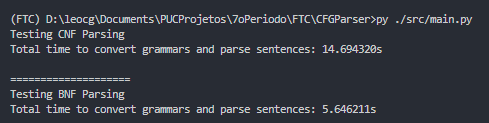
\includegraphics{parsing.png}
    \caption{Teste das gramáticas}
    \label{fig:parsing}
\end{figure}

% \section{Conclusão}

\bibliographystyle{sbc}
\bibliography{sbc-template}

\end{document}
